\documentclass[12pt]{article}
\usepackage{amsmath}
\usepackage{graphicx}
\usepackage{float}
\begin{document}
\title{Electrical Engineering 113, Homework 2}
\date{April 15th, 2019}
\author{Michael Wu\\UID: 404751542}
\maketitle

\newcommand*{\underuparrow}[1]{\underset{\uparrow}{#1}}

\section*{Problem 1}

\paragraph{a)}

This system is linear. Consider the following equations.
\begin{align*}
    x[n] &= Ax_1[n]+Bx_2[n]\\
    y_1[n] &=\frac{1}{M+1}\sum_{k=0}^M\lambda^kx_1[n-k]\\
    y_2[n] &=\frac{1}{M+1}\sum_{k=0}^M\lambda^kx_2[n-k]\\
    y[n]&=\frac{1}{M+1}\sum_{k=0}^M\lambda^kx[n-k]\\
    &=\frac{1}{M+1}\sum_{k=0}^M\lambda^k(Ax_1[n-k]+Bx_2[n-k])\\
    &=A\frac{1}{M+1}\sum_{k=0}^M\lambda^kx_1[n-k]+B\frac{1}{M+1}\sum_{k=0}^M\lambda^kx_2[n-k]\\
    &=Ay_1[n]+By_2[n]
\end{align*}
So a linear combination of inputs to the system results in a linear combination of outputs from the system.

This system is causal, since \(y[n]\) only depends on \(x[n-k]\) where \(k\geq0\). So \(n\geq n-k\), and
the output only depends on the past and present input.

This system is time invariant, since the only components of the output that depend on \(n\) are the \(x[n-k]\)
terms. If there is a delay in the input, there will be the same delay in the output.

This system is stable. If \(x[n]<A\) for some constant \(A\) and all \(n\), then we also have the following result.
\[y[n]=\frac{1}{M+1}\sum_{k=0}^M\lambda^kx[n-k]\leq\frac{A}{M+1}\sum_{k=0}^M\lambda^k<\frac{AM}{M+1}<A\]
So \(y[n]\) is also bounded and our system is stable.

\paragraph{b)}

This system is linear. Consider the following equations.
\begin{align*}
    x[n] &= Ax_1[n]+Bx_2[n]\\
    y_1[n] &=\frac{1}{|n|+1}x_1[-n^2]\\
    y_2[n] &=\frac{1}{|n|+1}x_2[-n^2]\\
    y[n]&=\frac{1}{|n|+1}x[-n^2]\\
    &=\frac{1}{|n|+1}(Ax_1[-n^2]+Bx_2[-n^2])\\
    &=A\frac{1}{|n|+1}x_1[-n^2]+B\frac{1}{|n|+1}x_2[-n^2]\\
    &=Ay_1[n]+By_2[n]
\end{align*}
So a linear combination of inputs to the system results in a linear combination of outputs from the system.

This system is also causal. At \(n\geq0\), \(x[-n^2]\) must occur either in the present or past since \(-n^2\) cannot be
positive and nonzero. At \(n<0\), \(x[-n^2]\) must occur in the present or past since \(|n^2|>|n|\).

This system is not time invariant. Consider \(x[n]=\delta[n]\). Then \(y[n]=\delta[n]\). But if \(x[n]=\delta[n-1]\),
then \(y[n]=0\neq\delta[n-1]\).

This system is stable. If \(x[n]<A\) for some constant \(A\) and all \(n\), then we also have the following result.
\[y[n]=\frac{1}{|n|+1}x[-n^2]\leq x[-n^2]<A\]
So \(y[n]\) is also bounded and our system is stable.

\section*{Problem 2}

We cannot say whether the system is time invariant or not, since a time invariant system must cause a delay in the
output for any corresponding delay in the input. We are given only two input and output pairs and do not know about
the behavior of the system for any arbitrary delay. The system could be the following linear time variant system.
\[y[n]=(u[n]x[n])*\frac{1}{2}(\delta[n]+u[n])\]
It could also be the following linear time invariant system.
\[y[n]=x[n]*\frac{1}{2}(\delta[n]+u[n])\]
These both produce the same responses for the given inputs, but the time variant version zeros out the section of the input
signal where \(n<0\). If we input \(x_1[n]=\delta[n]\) and \(x_2[n]=\delta[n+1]\) into the time variant system, we obtain
the outputs \(y_1[n]=\frac{1}{2}(\delta[n]+u[n])\) and \(y_2[n]=0\). Since these responses are not time shifted versions
of one another, the system is not time invariant.

\section*{Problem 3}

\paragraph{a)}

\begin{align*}
    \frac{y_a(t)-y_a(t-T)}{T}+Ay_a(t)&=Ax_a(t)\\
    \left(\frac{1}{T}+A\right)y_a(t)-\frac{y_a(t-T)}{T}&=Ax_a(t)\\
    \frac{1+TA}{T}y_a(t)&=Ax_a(t)+\frac{y_a(t-T)}{T}\\
    y_a(t)&=\frac{TAx_a(t)+y_a(t-T)}{1+TA}
\end{align*}

\paragraph{b)}

\begin{align*}
    y[n]&=\frac{TAx[n]+y[n-1]}{1+TA}\\
    &=\frac{1}{1+TA}y[n-1]+\frac{TA}{1+TA}x[n]\\
    &=\left(1-\frac{TA}{1+TA}\right)y[n-1]+\frac{TA}{1+TA}x[n]\\
    &=(1-\alpha)y[n-1]+\alpha x[n]\\
    \alpha&=\frac{TA}{1+TA}
\end{align*}

\section*{Problem 4}

\paragraph{a)}

\[x[n]*h[n]=\{0,1,3,4,\underuparrow{4},2,-2,-4,-4,-3,-1,0\}\]

\paragraph{b)}

Begin with the definition of convolution.
\[y[n]=x[n]*h[n]=\sum_{k=-\infty}^\infty x[k]h[n-k]\]
We can then show that a shift in \(x[n]\) results in a corresponding shift in the output.
\begin{align*}
    x[n-m]*h[n]&=\sum_{k=-\infty}^\infty x[k-m]h[n-k]\\
    &=\sum_{k^\prime=-\infty}^\infty x[k^\prime]h[n-k^\prime-m]\\
    &=\sum_{k^\prime=-\infty}^\infty x[k^\prime]h[(n-m)-k^\prime]\\
    &=y[n-m]
\end{align*}
We made the substitution \(k^\prime=k-m\). We can also show that a shift in \(h[n]\) results in a
corresponding shift in the output.
\begin{align*}
    x[n]*h[n-m]&=\sum_{k=-\infty}^\infty x[k]h[n-k-m]\\
    &=\sum_{k=-\infty}^\infty x[k]h[(n-m)-k]\\
    &=y[n-m]
\end{align*}

\section*{Problem 5}

\paragraph{a)}

\[h_{eq}[n]=h_1[n]+h_2[n]*(h_3[n]+h_4[n])\]

\paragraph{b)}

\begin{align*}
    h_{eq}[n]&=e^{-0.1n}u[n] + (u[n]-u[n-3])*(u[n]-u[n-3]+\delta[n-2])\\
    &=e^{-0.1n}u[n] + u[n]*u[n] - 2u[n]*u[n-3]\\
    &\qquad+ u[n-3]*u[n-3] + u[n-2] - u[n-5]\\
    &=e^{-0.1n}u[n] + (n+1)u[n] - 2(n-2)u[n-3]\\
    &\qquad+ (n-5)u[n-6] + u[n-2] - u[n-5]\\
    &=(e^{-0.1n}+n+1)u[n] + u[n-2] - 2(n-2)u[n-3]\\
    &\qquad- u[n-5] + (n-5)u[n-6]
\end{align*}

\paragraph{c)}

The output of the system when \(x[n]=u[n]\) is shown below..

\begin{figure}[H]
    \begin{center}
        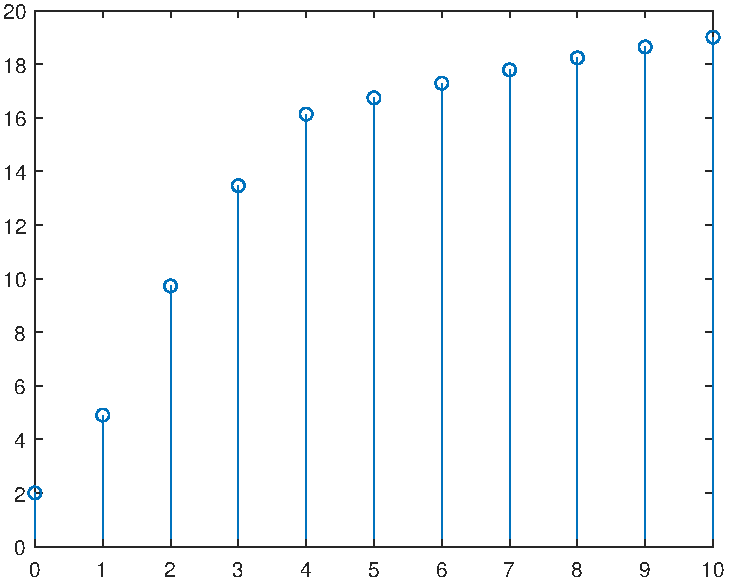
\includegraphics[width=2in]{problem5c.pdf}
    \end{center}
\end{figure}

\section*{Problem 6}

\paragraph{a)}

I upsampled the signal with the following line of code.
\begin{verbatim}
W = upsample(X,3);
\end{verbatim}
I implemented the moving average filter with the following line of code.
\begin{verbatim}
Y = smoothdata(W, 'movmean', window);
\end{verbatim}
Here \texttt{window} is a variable that controls the window size. When it is
1, the audio contains a high pitched buzzing that is an artifact of the upsampling,
since the audio data rapidly alternates between some value and zero. When it is 5, the
buzzing is slightly reduced in harshness but still present. At 10 the buzzing is again
reduced but still present. At 50 the buzzing is almost entirely gone, but the track
becomes very bass heavy since the higher frequencies are also reduced. The volume is also
lower. At 100 the track sounds like it's underwater. The attacks are very soft so the notes
blend together, it's very bass heavy, and the volume is further reduced. Depending on
the preferred effect and desired amount of bass, window sizes of 10, 50, or 100 would sound
good. Personally I would use a window size of 10 in order to maintain the voicing of the notes.

\paragraph{b)}

The transfer function for an exponential smoother can be solved in the following manner.
\begin{align*}
    y[n]&=(1-\alpha)y[n-1]+\alpha x[n]\\
    Y(z)&=(1-\alpha)z^{-1}Y(z)+\alpha X(z)\\
    (1+(\alpha-1)z^{-1})Y(z)&=\alpha X(z)\\
    \frac{Y(z)}{X(z)}&=\frac{\alpha}{1+(\alpha-1) z^{-1}}
\end{align*}
I implemented the exponential smoother with the following line of code.
\begin{verbatim}
Y = filter(alpha, [1 alpha-1], W);
\end{verbatim}
At \(\alpha=0\), the output was entirely zero and no sound played. At \(\alpha=1\), no
smoothing occurs and there is a high buzzing that is an artifact of the upsampling. At \(\alpha=0.8\),
this buzzing is still mostly present. At \(\alpha=0.5\), the buzzing is still present but the harshness
is reduced. The best value was \(\alpha=0.3\), since the other values of \(\alpha\) were too high
and let the signal drop to low values due to the zero entries. At \(\alpha=0.3\) the signal stays
at somewhat the same level so the buzzing is only slightly perceptible. Lowering \(\alpha\) even
further reduces the volume and reduced high frequencies, but it does not soften the attack of the notes
like the moving average filter.

\end{document}